%!TEX root = ../../thesis.tex

\section{Attribute Indexing}
\label{methodology:attribute_index}

Attribute indexing is a fundamental component of the FlatCityBuf format, enabling efficient filtering and retrieval of city objects based on their non-spatial properties. This section details the requirements, design considerations, and implementation of the attribute indexing system.

\subsection{Query Requirements Analysis}
\label{methodology:attribute_index:query_requirements}

The attribute indexing system in FlatCityBuf was designed to support query patterns commonly encountered in geospatial applications. To determine which query operators to prioritize, we analyzed established standards in the geospatial domain and common usage patterns in existing GIS software.

\subsubsection{Common Query Operators in Geospatial Standards}
\label{methodology:attribute_index:query_requirements:standards}

Two major OGC standards provide guidance on common query operators: Filter Encoding Standard \citep{ogc_filter_encoding_2010} and Common Query Language \citep{ogc_cql2_2024}. These standards define operators in several categories, as summarized in Table~\ref{tab:query_operators}.

\begin{table}[ht]
  \centering
  \caption{Common query operators in geospatial standards}
  \label{tab:query_operators}
  \begin{tabular}{p{3cm}p{5cm}p{5cm}}
    \hline
    \textbf{Category} & \textbf{OGC Filter Encoding} & \textbf{OGC CQL} \\
    \hline
    \textbf{Logical Operators} &
    AND, OR, NOT &
    AND, OR, NOT \\
    \hline
    \textbf{Comparison Operators} &
    PropertyIsEqualTo, PropertyIsNotEqualTo, PropertyIsLessThan, PropertyIsGreaterThan, PropertyIsLessThanOrEqualTo, PropertyIsGreaterThanOrEqualTo, PropertyIsLike, PropertyIsNull, PropertyIsBetween &
    $=$, $!=$, $<$, $<=$, $>$, $>=$, LIKE, IS NULL, BETWEEN, IN \\
    \hline
    \textbf{Spatial Operators} &
    BBOX, Equals, Disjoint, Touches, Within, Overlaps, Crosses, Intersects, Contains, DWithin, Beyond &
    INTERSECTS, EQUALS, DISJOINT, TOUCHES, WITHIN, OVERLAPS, CROSSES, CONTAINS \\
    \hline
    \textbf{Temporal Operators} &
    After, Before, Begins, BegunBy, During, TContains, TEquals, TOverlaps, Ends, EndedBy, Meets, MetBy, OverlappedBy, AnyInteracts &
    AFTER, BEFORE, BEGINS, BEGUNBY, DURING, TCONTAINS, TEQUALS, TOVERLAPS, ENDS, ENDEDBY, MEETS, METBY, OVERLAPPEDBY, ANYINTERACTS \\
    \hline
    \textbf{Additional Capabilities} &
    ResourceId &
    Functions, Arithmetic Expressions, Array Operators \\
    \hline
  \end{tabular}
\end{table}

\subsubsection{Priority Operators for FlatCityBuf}
\label{methodology:attribute_index:query_requirements:priorities}

Based on this analysis and the practical constraints of optimizing for cloud-based access, FlatCityBuf prioritizes support for the following operators:

\begin{enumerate}
  \item \textbf{Primary Comparison Operators}: Operators with direct index support
    \begin{itemize}
      \item Equality ($=$)
      \item Inequality ($!=$)
      \item Less than ($<$)
      \item Less than or equal ($<=$)
      \item Greater than ($>$)
      \item Greater than or equal ($>=$)
      \item BETWEEN (implemented as combined $\geq$ and $\leq$)
    \end{itemize}

  \item \textbf{Logical Combinations}: Supported at the query execution level
    \begin{itemize}
      \item AND (intersection of result sets)
      \item OR (union of result sets) (This will be implemented in the future)
    \end{itemize}

    \todo{Uncomment if I could finish the implementation}
    %   \item \textbf{Spatial Filtering}: Integrated with attribute filtering
    %     \begin{itemize}
    %       \item BBOX (bounding box intersection)
    %     \end{itemize}
\end{enumerate}

Other operators from the standards were evaluated but not prioritized in the initial implementation, either because they require more complex index structures (\eg, LIKE operators) or are less commonly used in typical 3D city model queries.

By focusing on these high-priority operators, FlatCityBuf's attribute indexing system aims to support the most common query patterns while maintaining efficient performance for cloud-based access. This approach provides capabilities that exceed current offerings such as the 3DBAG API, which primarily supports feature retrieval by identification attribute (\texttt{identificatie}) and is still working toward full OGC compliance \citep{3dbag_api_2023}.

\subsection{\texorpdfstring{\ac{s+tree}}{S+tree} Design and Modifications}
\label{methodology:attribute_index:static_btree_design}

After evaluating alternatives, a \ac{s+tree} with significant modifications was adopted for FlatCityBuf's attribute indexing. \ac{s+tree} is a variant of the Static B+Tree that is specialised for read-only access patterns. Its theoretical background is described in \autoref{tb:static_btree}. This decision was based on the following considerations:

\begin{itemize}
  \item \textbf{\ac{io} Efficiency and Balanced Performance}: B+trees organise data into fixed-size nodes matching common CPU cache sizes, offering $O(\log_B n)$ search complexity where $B$ is the branching factor. This significantly reduces both the number of \ac{io} operations and network roundtrips compared to binary search, making it ideal for HTTP Range Requests where each roundtrip incurs substantial latency.

  \item \textbf{Query Versatility}: Unlike specialized data structures such as hash tables (optimized for exact matches) or sorted arrays (better for range queries), the B+tree structure efficiently supports both exact match and range queries without compromising performance in either case. This versatility makes it well-suited for the diverse query patterns common in 3D city model applications.
\end{itemize}

\subsubsection{\ac{s+tree} Characteristics}
\label{methodology:attribute_index:static_btree_characteristics}

A \ac{s+tree} differs from a traditional B+tree in several important aspects:

\begin{itemize}
  \item \textbf{Immutability}: Once constructed, the tree structure remains fixed, eliminating the need for complex rebalancing operations.

  \item \textbf{Perfect Node Fill}: All nodes except possibly the rightmost nodes at each level are filled to capacity, maximizing space efficiency.

  \item \textbf{Predictable Structure}: The tree shape is determined solely by the number of elements and the node size, making navigation more efficient.

  \item \textbf{Bulk Construction}: The tree is built bottom-up in a single pass from sorted data, rather than through incremental insertions.
\end{itemize}

The original S+tree algorithm as described by \citet{static_b_trees} provides an excellent foundation for read-only indexing. However, several significant modifications were necessary to adapt it to the specific requirements of FlatCityBuf:

\begin{itemize}
  \item \textbf{Duplicate Key Handling}: 3D city model attributes often contain numerous duplicate values (\eg, hundreds of features with "Delft" as the value for "city name"). The \ac{s+tree} implementation described in literature \citep{static_b_trees} does not address the case of having duplicate values. The modified implementation incorporates a dedicated payload section that efficiently stores multiple feature references for identical attribute values without compromising the tree structure or search performance.

    For handling duplicate keys in indexing structures, \citet{ramez_2015} outlines three main approaches: (1) including duplicate entries in the index, (2) using variable-length records with a repeating pointer field, or (3) keeping fixed-length index entries with a single entry per key value and an extra level of indirection to handle multiple pointers. FlatCityBuf adopts the third approach, which is "more commonly used" according to \citet{ramez_2015}, by implementing a payload section that stores the collection of feature offsets for each duplicate key. This design choice was made to maintain a simple implementation for search algorithms while efficiently handling attributes with potentially high duplicate cardinality. The fixed-length entries in the tree structure preserve the binary search efficiency, while the separate payload section accommodates the variable number of references without complicating the tree traversal logic.

  \item \textbf{Multi-type Support}: The index structure was extended to handle various attribute data types commonly found in 3D city models, including numeric types (integers, floating-point), string values, boolean flags, and temporal data (dates, timestamps).

  \item \textbf{Explicit Node Offsets}: While the original S+tree uses mathematical calculations to determine node positions, FlatCityBuf's implementation stores explicit byte offsets to child nodes. This modification simplifies the implementation without compromising performance. The parent node item has a 64-bit offset to the first child item of left child node.

  \item \textbf{Payload Pointer Mechanism}: To efficiently handle duplicate keys, the implementation uses a tag bit in the offset value to distinguish between direct feature references and pointers to the payload section. When the most significant bit is set, the remaining bits encode an offset to the payload section where multiple feature offsets are stored consecutively. This approach minimizes both the storage overhead and redundant HTTP requests for unique keys while enabling support for duplicate keys.

\end{itemize}

These modifications ensure that the S+tree implementation is optimized for the specific characteristics of 3D city model data while preserving the performance advantages of the original algorithm.

\subsection{Attribute Index Implementation}
\label{methodology:attribute_index:implementation}

The attribute indexing system in FlatCityBuf is implemented as a binary encoded structure with four main components:

\begin{enumerate}
  \item \textbf{Index Metadata}: Contains metadata about the index, including the column being indexed, branching factor, and number of unique values. This is stored in the header section of the file \autoref{methodology:header:schema_indexing}.
  \item \textbf{Tree Structure}: A hierarchical arrangement of nodes with keys and pointers. Though it's called as "tree", it's conceptual structure. The actual structure is a linear sequence of nodes. Both internal and leaf nodes are stored consecutively in the "flat" structure.
  \item \textbf{Payload Section}: Stores arrays of feature offsets for duplicate key values. Each payload entry has a 32-bit length prefix that indicates the number of feature offsets that follow.
\end{enumerate}

\begin{figure}[htbp]
  \centering
  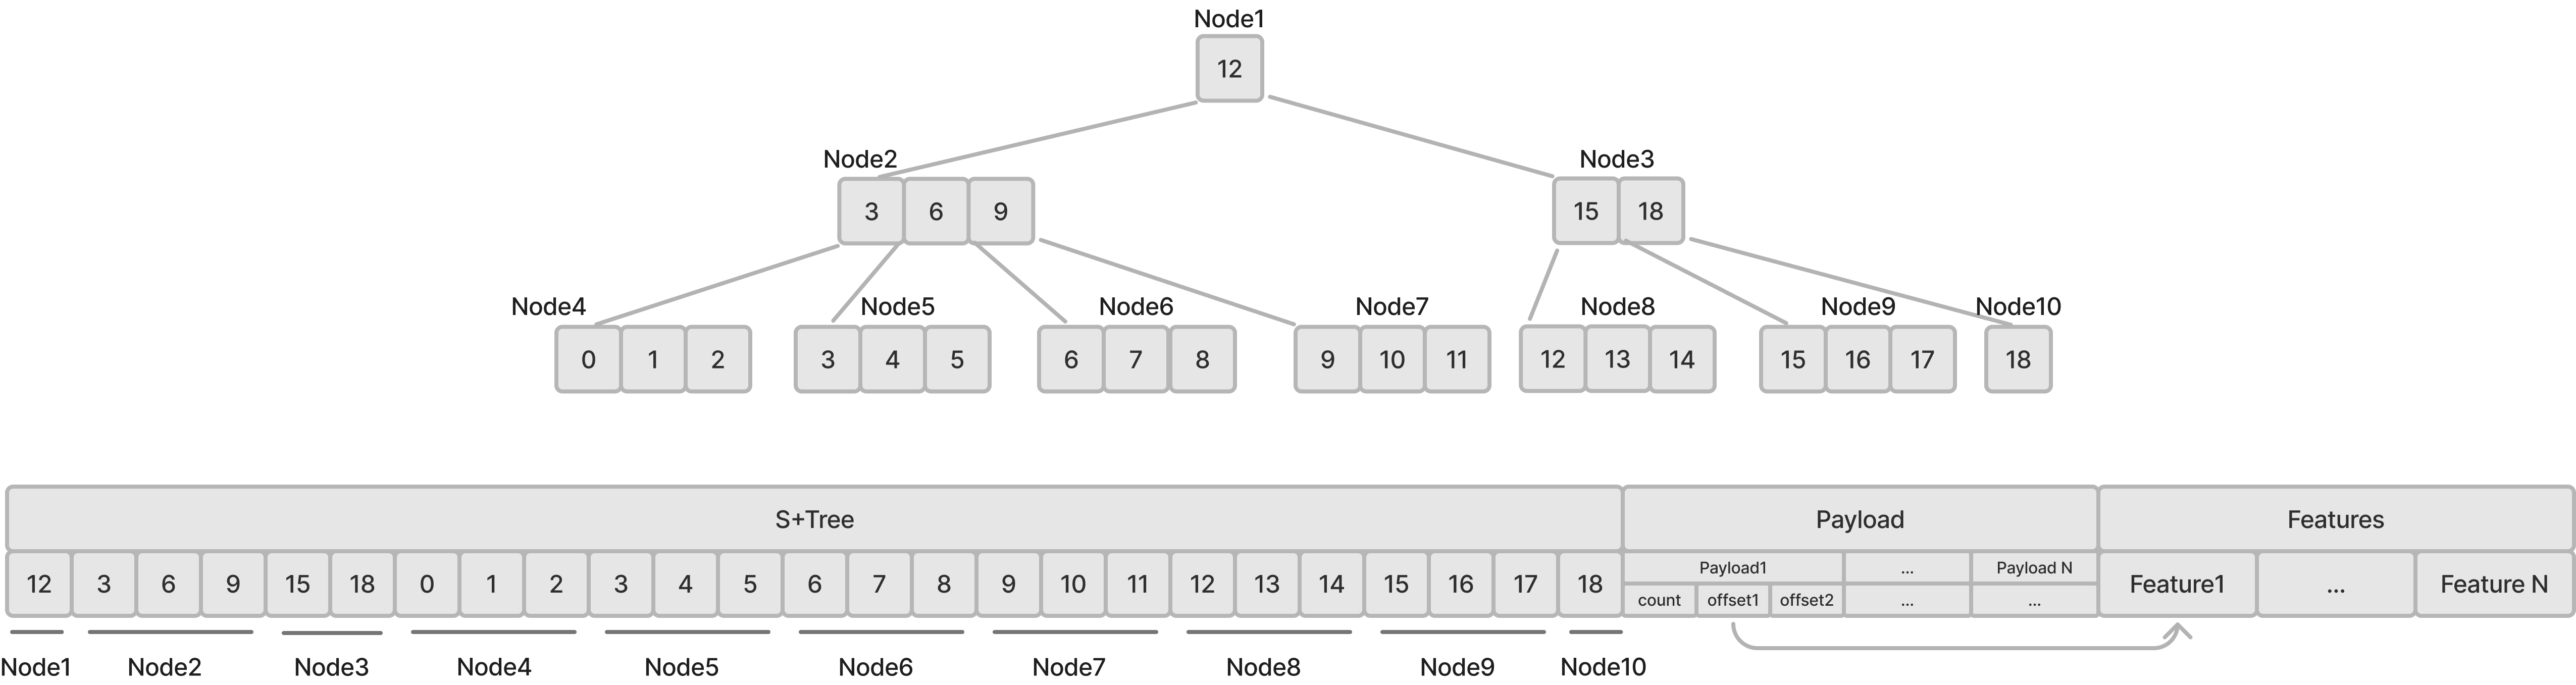
\includegraphics[width=0.8\textwidth]{figs/methodology/attribute_index.png}
  \caption{Attribute index implementation in FlatCityBuf}
  \label{fig:methodology:attribute_index}
\end{figure}

\subsection{Construction of the Attribute Index}
\label{methodology:attribute_index:construction}

The construction of the attribute index follows these processes:

\begin{enumerate}
  \item Create pairs of attribute values and their corresponding feature offsets.
  \item Sort the pairs by the attribute values.
  \item Create the payload section by grouping the feature offsets for duplicate attribute values.
  \item Build the tree structure with configuration of branching factor and the number of unique values. (This determines the height of the tree and the range of array for each level of the tree)
    \begin{itemize}
      \item Leaf nodes: $\text{branching factor} - 1$ items are grouped together as one leaf node. Each item has a key and a u64 offset to either the feature or payload section.
      \item Internal nodes: branching factor items are grouped together as one internal node. The key value of an internal node is the minimum key of the subtree of its right child node.
    \end{itemize}
  \item Structure the tree from bottom to top and write it to the file in the order from top to bottom.
\end{enumerate}

\subsection{Serialization of Keys in the Tree}
\label{methodology:attribute_index:key_serialization}

Key serialization in the attribute index is a critical aspect of the implementation, directly affecting both storage efficiency and query performance. FlatCityBuf implements type-specific serialization strategies that balance storage requirements, comparison efficiency, and implementation complexity.

\subsubsection{Fixed-Length Value Serialization}
\label{methodology:attribute_index:fixed_length_serialization}

Fixed-length values offer significant advantages for tree structures, enabling predictable node sizes and efficient binary search within nodes. FlatCityBuf serializes fixed-length values using the following strategies:

\begin{itemize}
  \item \textbf{Integer Types}: Primitive integer types (i8, i16, i32, i64, u8, u16, u32, u64) are serialized directly in their native binary format using little-endian byte order. For example, a u64 value occupies exactly 8 bytes in the index structure.

  \item \textbf{Floating-Point Types}: IEEE 754 floating-point values \citep{ieee_754_2023} use their native binary representation, with special handling for NaN values to ensure consistent ordering semantics. This is implemented using the OrderedFloat wrapper type, which provides total ordering for floating-point values while preserving their binary efficiency.

  \item \textbf{Temporal Types}: Date and timestamp values are serialized using a normalized representation that preserves chronological ordering. Timestamps are encoded as a composite of two components: an i64 representing seconds since the epoch, followed by a u32 representing nanosecond precision, both in little-endian order. This 12-byte representation supports the full range of ISO 8601 datetime values with timezone information \citep{iso_8601_2023}.

  \item \textbf{Boolean Values}: Boolean values are encoded as a single byte (0 for false, 1 for true), aligning with common binary encodings while ensuring consistent sort order.
\end{itemize}

This direct serialization approach for fixed-length types minimizes both computational overhead during tree traversal and storage requirements in the index structure.

\subsubsection{Variable-Length Value Serialization}
\label{methodology:attribute_index:variable_length_serialization}

Supporting variable-length keys in B+tree structures presents significant implementation challenges. As \citet{ramez_2015} notes, variable-length keys can lead to unpredictable node sizes and uneven fan-out, complicating both the tree construction and traversal algorithms. This issue is particularly relevant for string attributes in 3D city models, where key lengths can vary substantially.

Modern database systems typically address this challenge through techniques such as prefix compression, where only the distinguishing prefix of each key is stored in non-leaf nodes. For example, when indexing last names, a non-leaf node might store only "Nac" and "Nay" as the discriminating prefixes between "Nachamkin" and "Nayuddin" \citep{ramez_2015}.

While implementing a full prefix compression scheme would be ideal, it would significantly increase the complexity of both the indexing algorithm and the format specification. After evaluating the trade-offs between implementation complexity and the practical requirements of 3D city model attribute data, FlatCityBuf adopts a pragmatic approach using fixed-length strings with a maximum length of 50 bytes. This length was selected based on analysis of common attribute values in 3D city datasets, where typical string attributes such as identifiers ("NL.IMBAG.Pand.0363100012345678"), city names ("Delft"), building types ("residential"), and similar values rarely exceed this length.

For strings shorter than the fixed length, padding with space characters ensures consistent key sizes throughout the tree structure. This approach simplifies implementation while still supporting the most common use cases found in 3D city model datasets. The space overhead from padding is generally acceptable given the relative infrequency of string attributes compared to numeric attributes in typical datasets.

\subsection{Query Strategies}
\label{methodology:attribute_index:query_strategies}

The attribute index implementation provides two core functions that enable efficient query execution:

\begin{itemize}
  \item \textbf{find\_exact\_match}: Traverses the tree structure to locate an exact match for a specified key value.
  \item \textbf{find\_partition\_point}: Identifies the boundary positions within the tree for a given query value, essential for range-based operations.
\end{itemize}

These fundamental functions support both exact match and range queries. Range queries are implemented by determining lower and upper bounds using \texttt{find\_partition\_point} and then retrieving all results within those boundaries. For inequality queries, the implementation uses \texttt{find\_exact\_match} to identify the target item and then returns all items except the matched one. This query functionality aligns with the standard operators defined in \citet{ogc_filter_encoding_2010}:

\begin{itemize}
  \item \texttt{PropertyIsEqualTo}
  \item \texttt{PropertyIsNotEqualTo}
  \item \texttt{PropertyIsLessThan}
  \item \texttt{PropertyIsGreaterThan}
  \item \texttt{PropertyIsLessThanOrEqualTo}
  \item \texttt{PropertyIsGreaterThanOrEqualTo}
  \item \texttt{PropertyIsBetween}
\end{itemize}

For complex logical operations, the implementation supports compound queries by executing multiple index lookups and combining the results. For \texttt{AND} operations, it computes the intersection of result sets, while \texttt{OR} operations would use the union of results. Currently, only the \texttt{AND} logical operator is fully implemented.

\subsection{Streaming \texorpdfstring{\ac{s+tree}}{S+tree} over HTTP}
\label{methodology:attribute_index:streaming_s_tree}

The index is structured to optimize for HTTP Range Requests, with several techniques employed to minimize network overhead:

\begin{itemize}
  \item \textbf{Streaming search}: The search algorithm operates in a streaming fashion, requesting only the nodes necessary for query evaluation in sequential order. This approach ensures that even with large indices, the system avoids loading the entire tree structure into memory, significantly reducing resource requirements.
  \item \textbf{Payload Prefetching}: Proactively caches parts of the payload section during initial query execution, reducing HTTP requests for duplicate keys.
  \item \textbf{Batch Payload Resolution}: Collects multiple payload references during tree traversal and resolves them with consolidated HTTP requests.
  \item \textbf{Request Batching}: Groups adjacent node requests to minimise network roundtrips.
  \item \textbf{Block Alignment}: Nodes are aligned to fixed size boundaries to match typical file system and HTTP caching patterns.
\end{itemize}

During query execution, the system interprets the provided condition (\eg, \texttt{building\_height > 25}) and traverses the appropriate attribute index to find matching features. The search algorithm adapts based on the condition type, using different traversal strategies for exact matches versus range queries. Results are returned as a set of feature offsets, which can then be used to retrieve the actual feature data from the features section of the file.
